\subsection{Integrated deformation}\label{sec:strain}
This benchmark is composed by 4 experiments characterised by different velocities imposed. For all the experiment the domain is 
a square of size $L_x=L_y=1$, discretised by $40\times 40$ elements. The velocities for the 4 experiments are imposed as follows:
\begin{itemize}
    \item Experiment 1: $u(x,y)=0$; $v(x,y)={\rm erf}[A(x-L_x/2)]$
    \item Experiment 2: $u(x,y)=0$; $v(x,y)=y$
    \item Experiment 3: $u(x,y)=y$; $v(x,y)=x$
    \item Experiment 4: $u(x,y)=2(-x+L_x/2)$; $v(x,y)=y-L_y/2$
\end{itemize}
The simulations are performed for $51$ timesteps, calculated by using CFL=$0.2$. The results show that the classic strain accumulation (old) is an acceptable approximation for small deformations only, while for increasing deformation a number of problems arise:
\begin{itemize}
    \item principal axes do not rotate for simple shear;
    \item negative principal strains can decrease below the theoretical limit of -1;
    \item the maximum shear deviates from the correct value.
\end{itemize}
These problems are solved by using the integrated deformation (new), as shown by the 4 experiments (Fig. \ref{fig:strain}).
All data can be found \href{https://github.com/cedrict/fieldstone/tree/master/images/stokes_sphere2D}{here}.

\begin{figure}[h!]
\centering
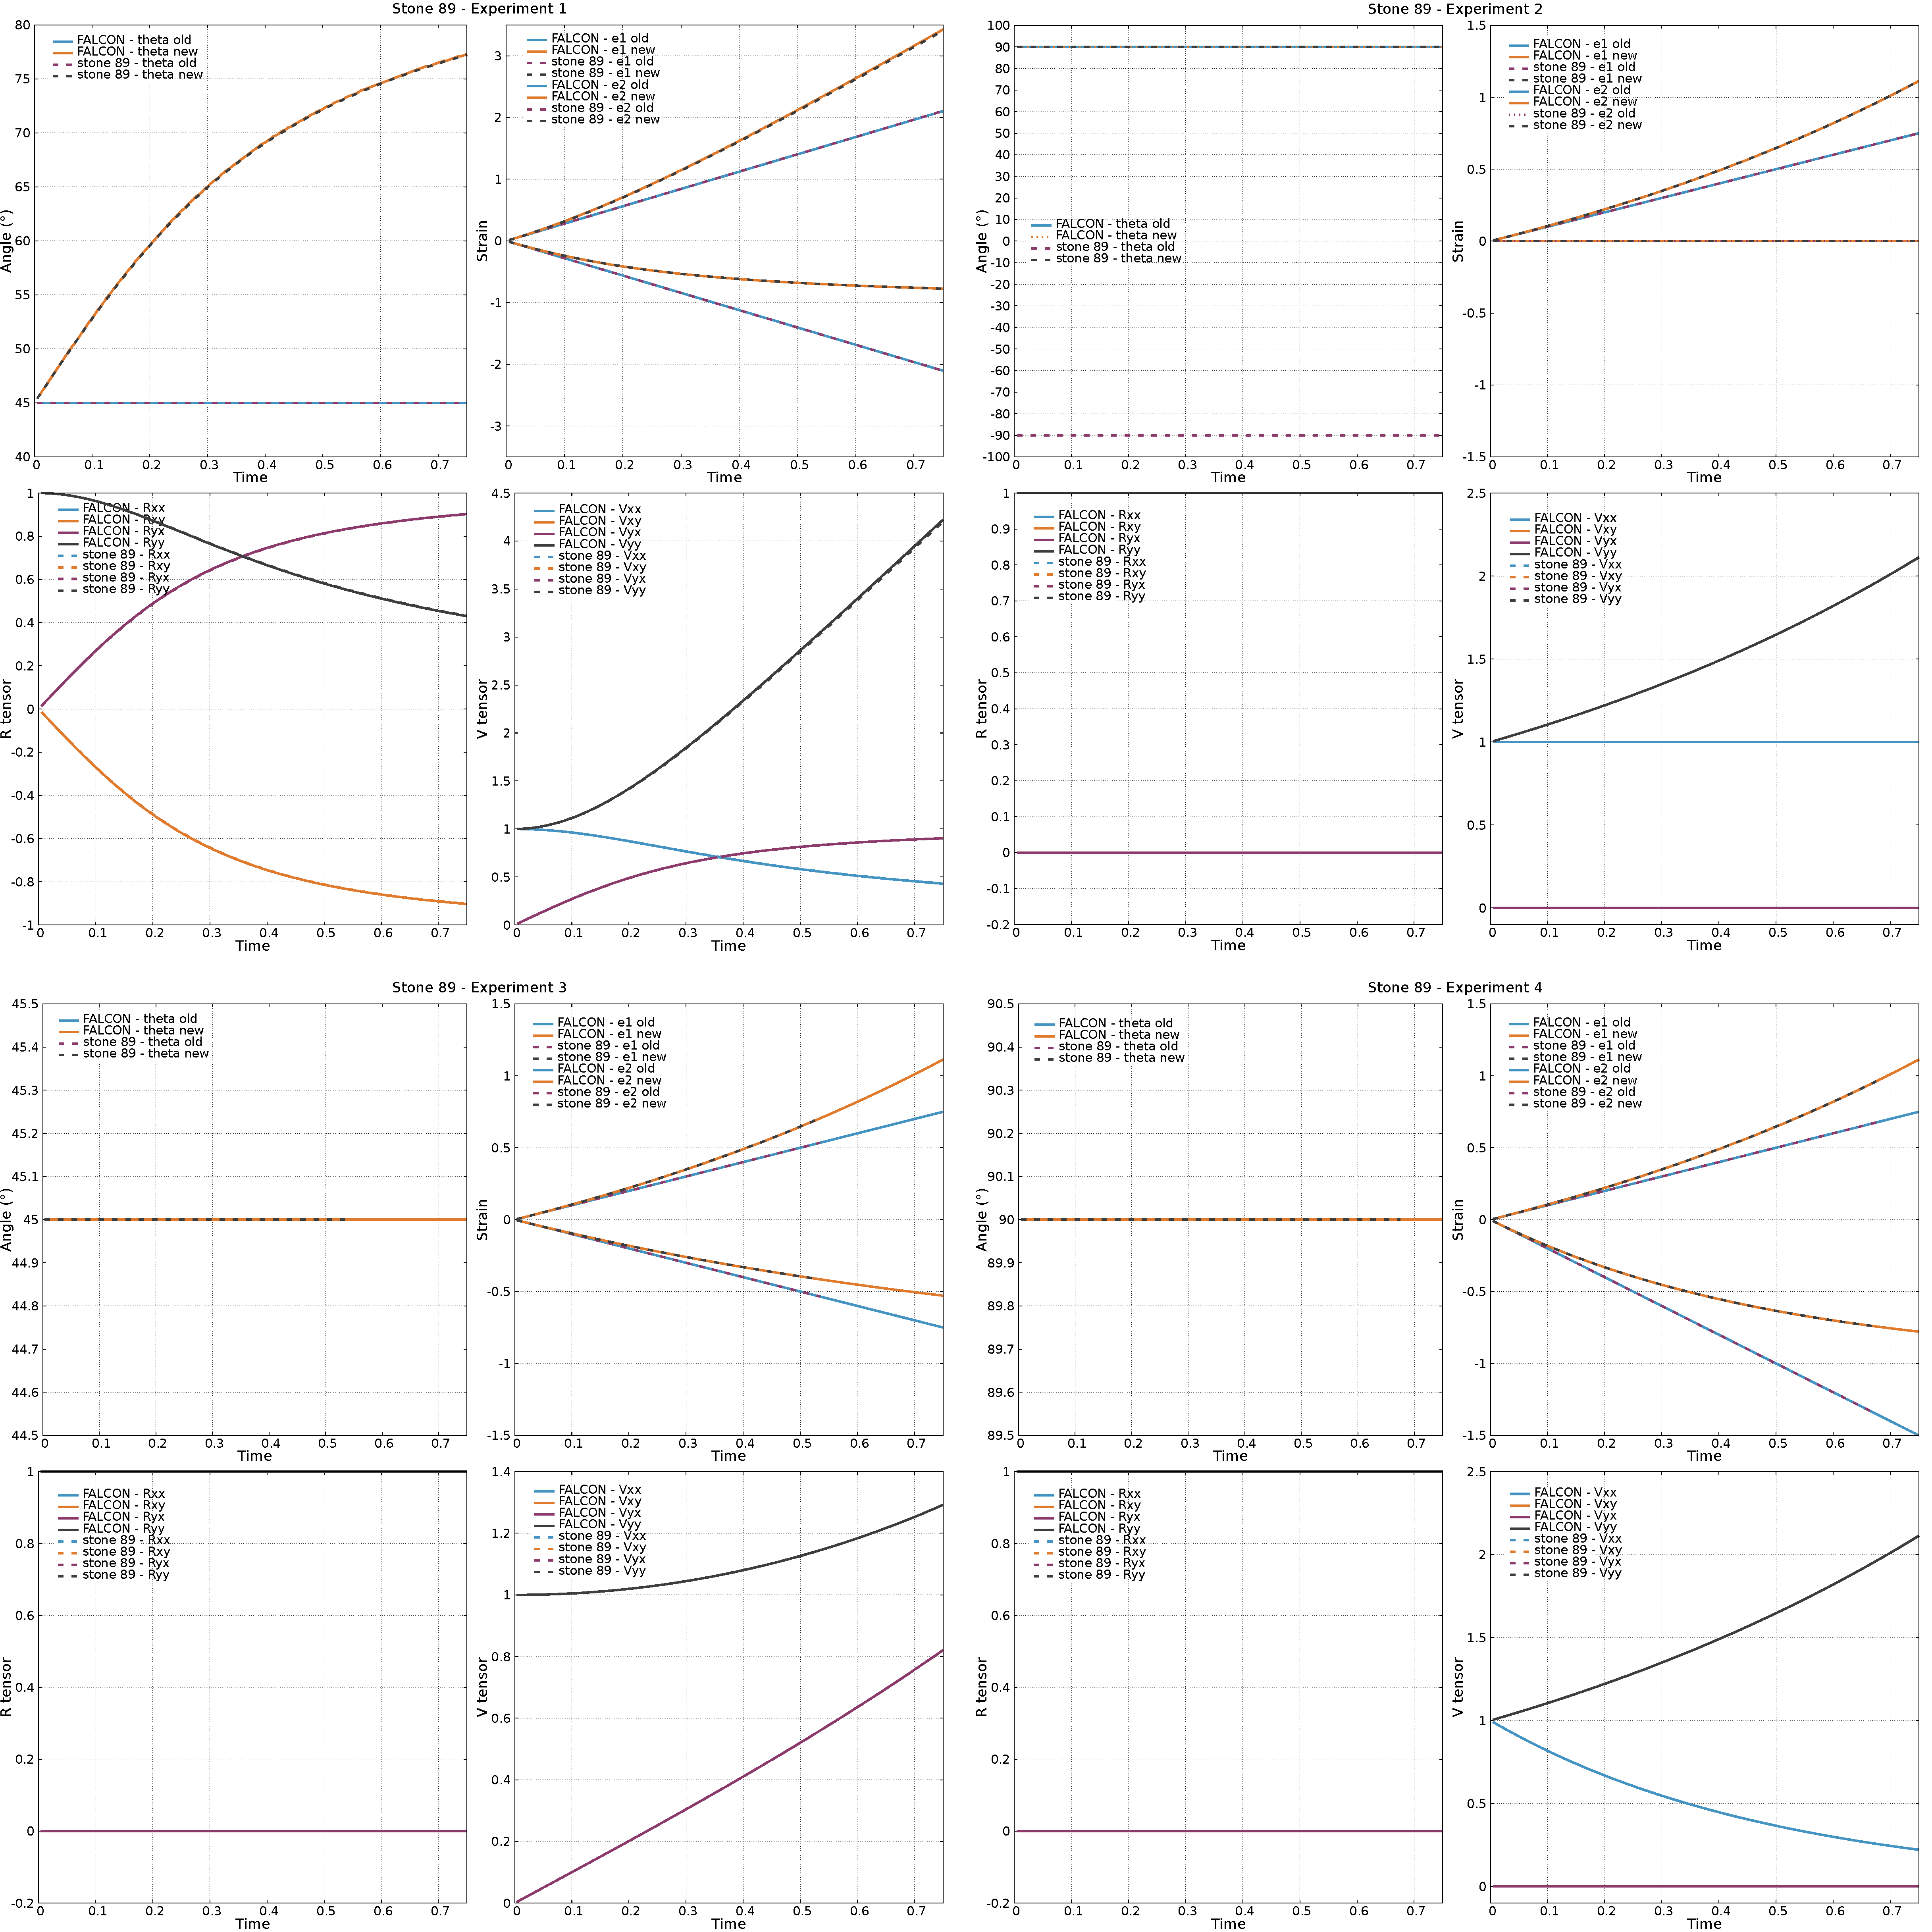
\includegraphics[width=17.5cm]{./Figures/stone_89_exp_all.pdf}
\caption{Comparison of angle and principal strains for the 4 experiments between the classic method (old, continuous blue and dashed purple lines) and the integrated deformation (new, continuous orange and dashed black lines). In addition, the values for the $\textbf{R}$ and $\textbf{V}$ matrices calculated with the new method are shown. Results are compared with those obtained in \href{https://surfdrive.surf.nl/s/G5zXEmS4zh5qutY?dir=/&editing=false&openfile=true}{Stone 89}.}
\label{fig:strain}
\end{figure}